\section{Stresses}
\subsection*{Internal Forces}
\smallskip

Internal cohesive forces are at the origin of the stresses responsible for deformations. Modeling of these forces requires 2 hypotheses: \\

\begin{enumerate}
\item Cohesive force distributed over the surface $\partial \omega$ of the sub-domain
\item Nominal stress vector only depends on the orientation of the surface in $\underline{\mathbf{x}} \rightarrow$ because PK1 is measured in original configuration! 
\end{enumerate}


\subsection*{Stresses}
\smallskip

\fbox{%
    \parbox{\columnwidth}{%
\textbf{Nominal stress tensor:} \hspace{8mm} Piola-Kirchhof 1 ($\underline{\underline{\mathbf{P}}}$)\\
\textbf{Spatial stress tensor:} \hspace{10mm} Cauchy (true) ($\underline{\underline{\mathbf{T}}}$)\\
\textbf{Material stress tensor:} \hspace{8mm} Piola-Kirchhof 2 ($\underline{\underline{\mathbf{S}}}$)
    }%
}

\begin{center}
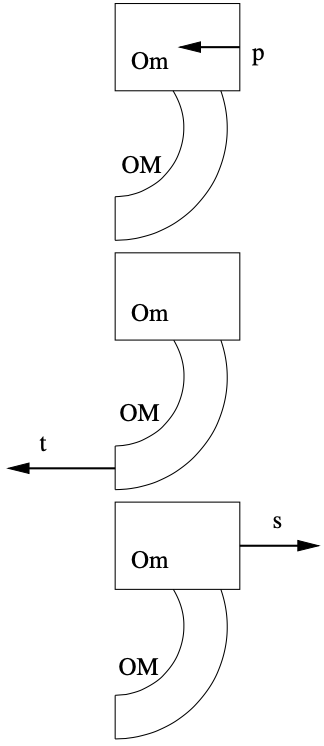
\includegraphics[width=0.3\linewidth]{img/StressVectors} \\
\end{center}

\textbf{Nominal stress tensor:} $ \underline{p} = \underline{\underline{P}} (\underline{x},t) \underline{n}(\underline{x})$ Where $\underline{\underline{P}} \neq$ symm! \\

\textbf{Spatial stress tensor:} (=Cauchy stress tensor)\\
$ \underline{\underline{T}} = J^{-1} \underline{\underline{P}} \underline{\underline{F}}^T$ \\
$ \underline{\underline{P}} = \underline{\underline{T}} \underline{\underline{F}}^*$ \\
$ = \underline{\underline{T}} \det(\underline{\underline{F}}) \cdot \underline{\underline{F}}^{-T}$

Nominal and Cauchy stress tensors are sensitive to rotations. \\
\textbf{Rates are NOT objective} \\


\textbf{Material stress tensor:} symmetric, objective, filters rigid body motions \\
$ \underline{\underline{\mathbf{P}}}(\underline{x}, t) = \underline{\underline{\mathbf{F}}}(\underline{x}, t) \underline{\underline{\mathbf{S}}}(\underline{x}, t)$ \\
3 invariants: \\
$I_1 = \Tr{\underline{\underline{S}}} = \sigma_1 + \sigma_2 + \sigma_3$ \\
$I_2 = \Sec{\underline{\underline{S}}} = \sigma_{2}\sigma_3 + \sigma_3\sigma_1 + \sigma_1\sigma_2 $ \\
$I_3 = \det{\underline{\underline{S}}} = \sigma_1\sigma_2\sigma_3$\\

\textbf{Stress tensors:} \\
$\underline{\underline{T}} = J^{-1} \underline{\underline{F}} \underline{\underline{S}} \underline{\underline{F}}^T$ \\
$\underline{\underline{S}} = J \underline{\underline{F}}^{-1} \underline{\underline{T}} \underline{\underline{F}}^{-T}$

Decompose \textbf{Stress tensor} in \textbf{Hydrostatic} and \textbf{Deviatoric} parts: \\
$\underline{\underline{\mathbf{S}}} = \underbrace{\frac{1}{3} \Tr{\underline{\underline{S}}}}_{\text{Hydr. P}} \underline{\underline{I}} + \underbrace{\underline{\underline{S}}'}_{\text{deviatoric part}}$ \\

\textbf{Stress deviator}: \\
$\underline{\underline{\mathbf{S}}}' = \underline{\underline{\mathbf{S}}} - \frac{1}{3}\Tr({\underline{\underline{\mathbf{S}}}}) \underline{\underline{\mathbf{I}}}$ \\

\textbf{Invariants of stress deviator}: \\
\begin{enumerate}
\item $J_1 = \Tr({\underline{\underline{\mathbf{S}}}}') = 0$
\item $J_2 = \frac{1}{2} \Tr({\underline{\underline{\mathbf{S}}}}'^2) = 0$
\item $J_3 = \frac{1}{3} \Tr({\underline{\underline{\mathbf{S}}}}'^3) = 0$
\end{enumerate}

\textbf{Von Mises stress:} Norm of the deviatoric part of the stress \\
$\tensor[^{vM}]{S}{} = \sqrt{\frac{3}{2} \underline{\underline{\mathbf{S'}}} : \underline{\underline{\mathbf{S'}}}} = \sqrt{3 J_2} = \sqrt{\frac{3}{2} \Tr({\underline{\underline{\mathbf{S}}}}'^2)}$ \\
With $\underline{\underline{\mathbf{S'}}} = \underline{\underline{\mathbf{S}}} + \pi \underline{\underline{\mathbf{I}}}$

\textbf{Hydrostatic Pressure:} $\pi = - \frac{1}{3} \operatorname{tr}\underline{\underline{\mathbf{T}}}$